\section{Implementation}
\label{sec:impl}

\subsection{External interface}
\begin{figure}[!htbp]
    \centerline{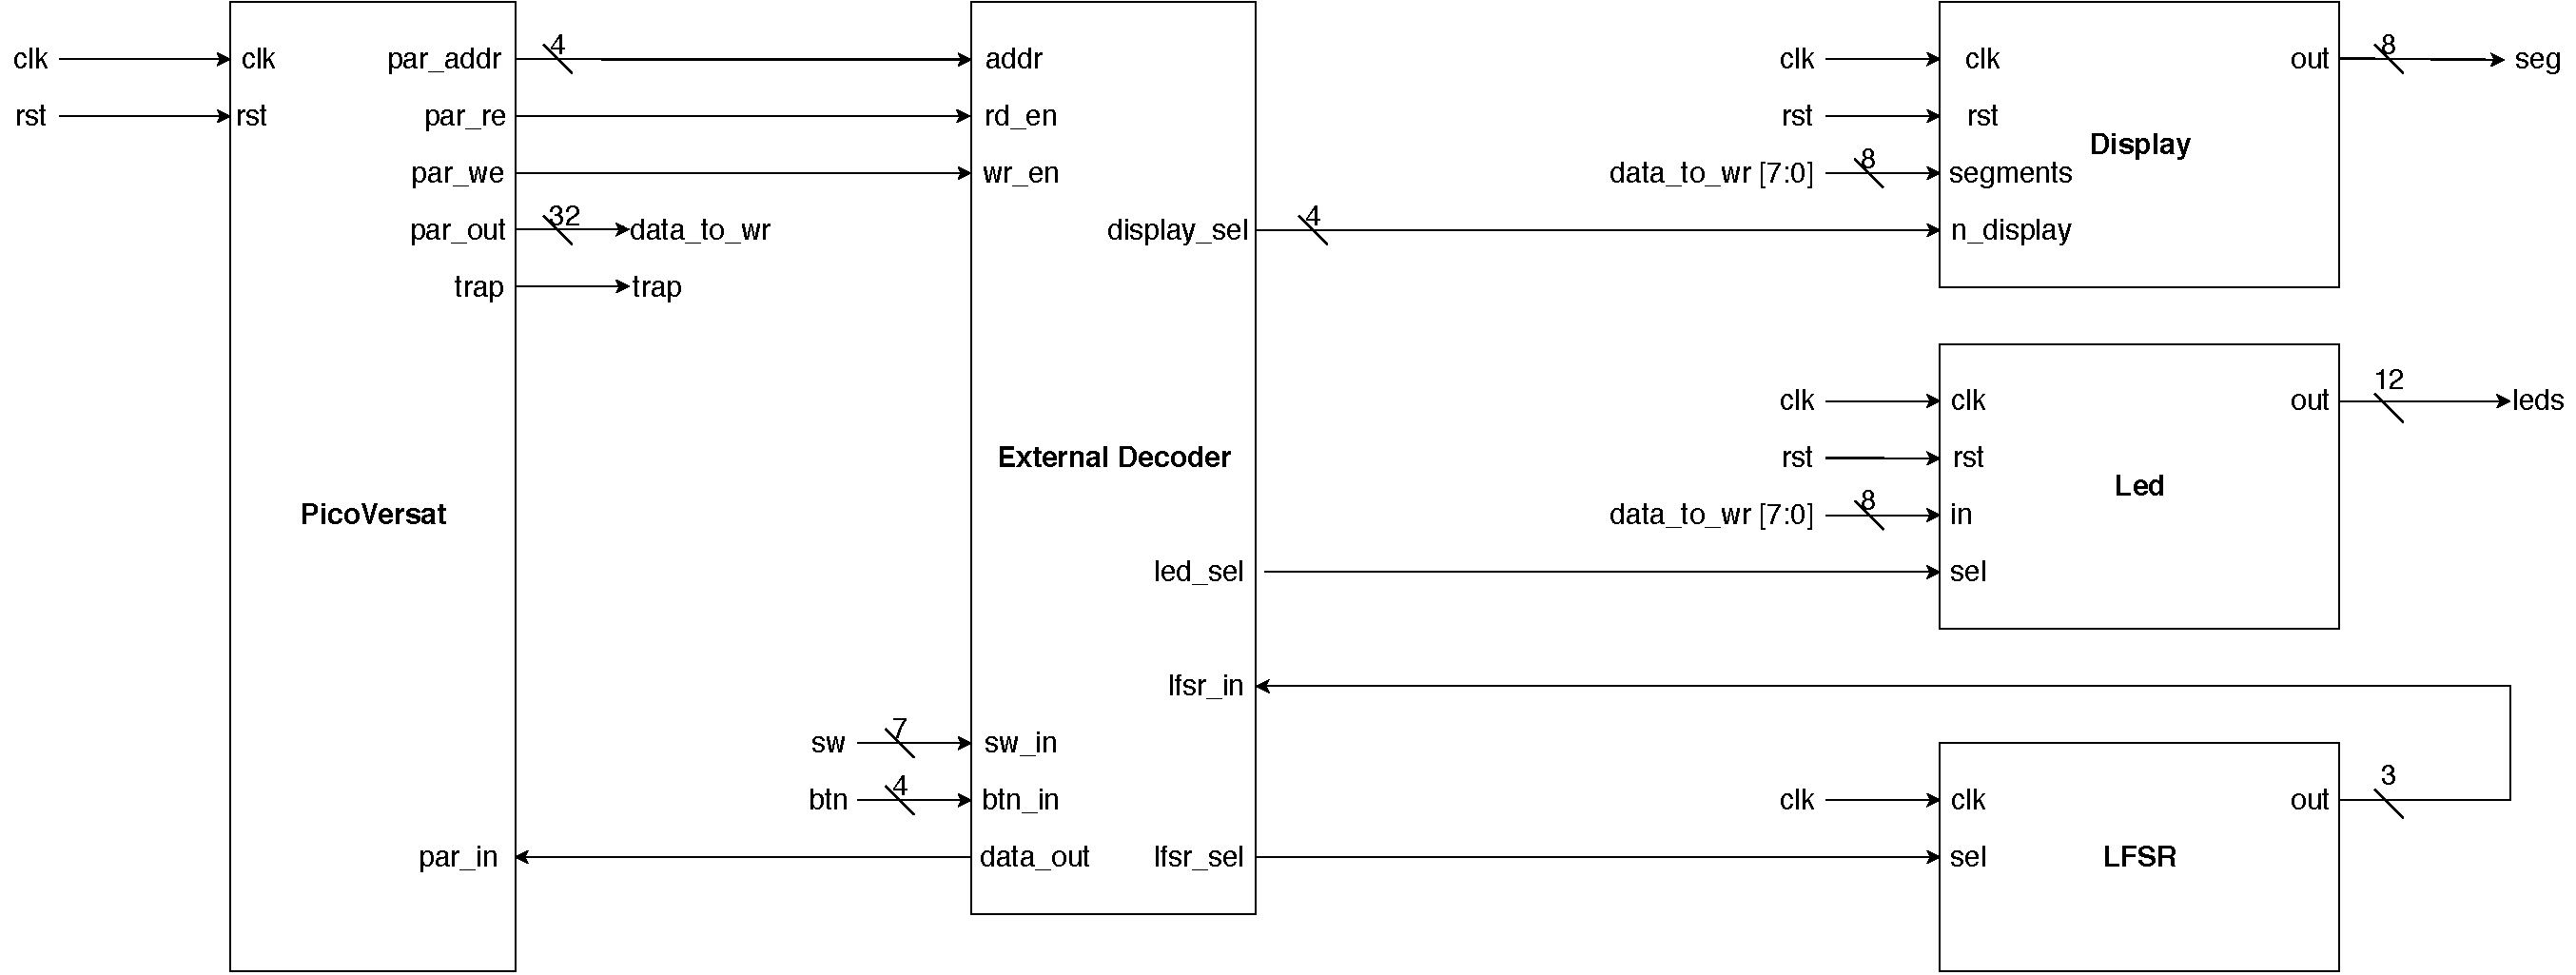
\includegraphics[scale=0.4]{ext_interface}}
    \vspace{0cm}\caption{External interface block diagram.}
    \label{fig:ext_interface}
\end{figure}

\clearpage
\subsection{Description of the display peripheral}
\begin{figure}[!htbp]
    \centerline{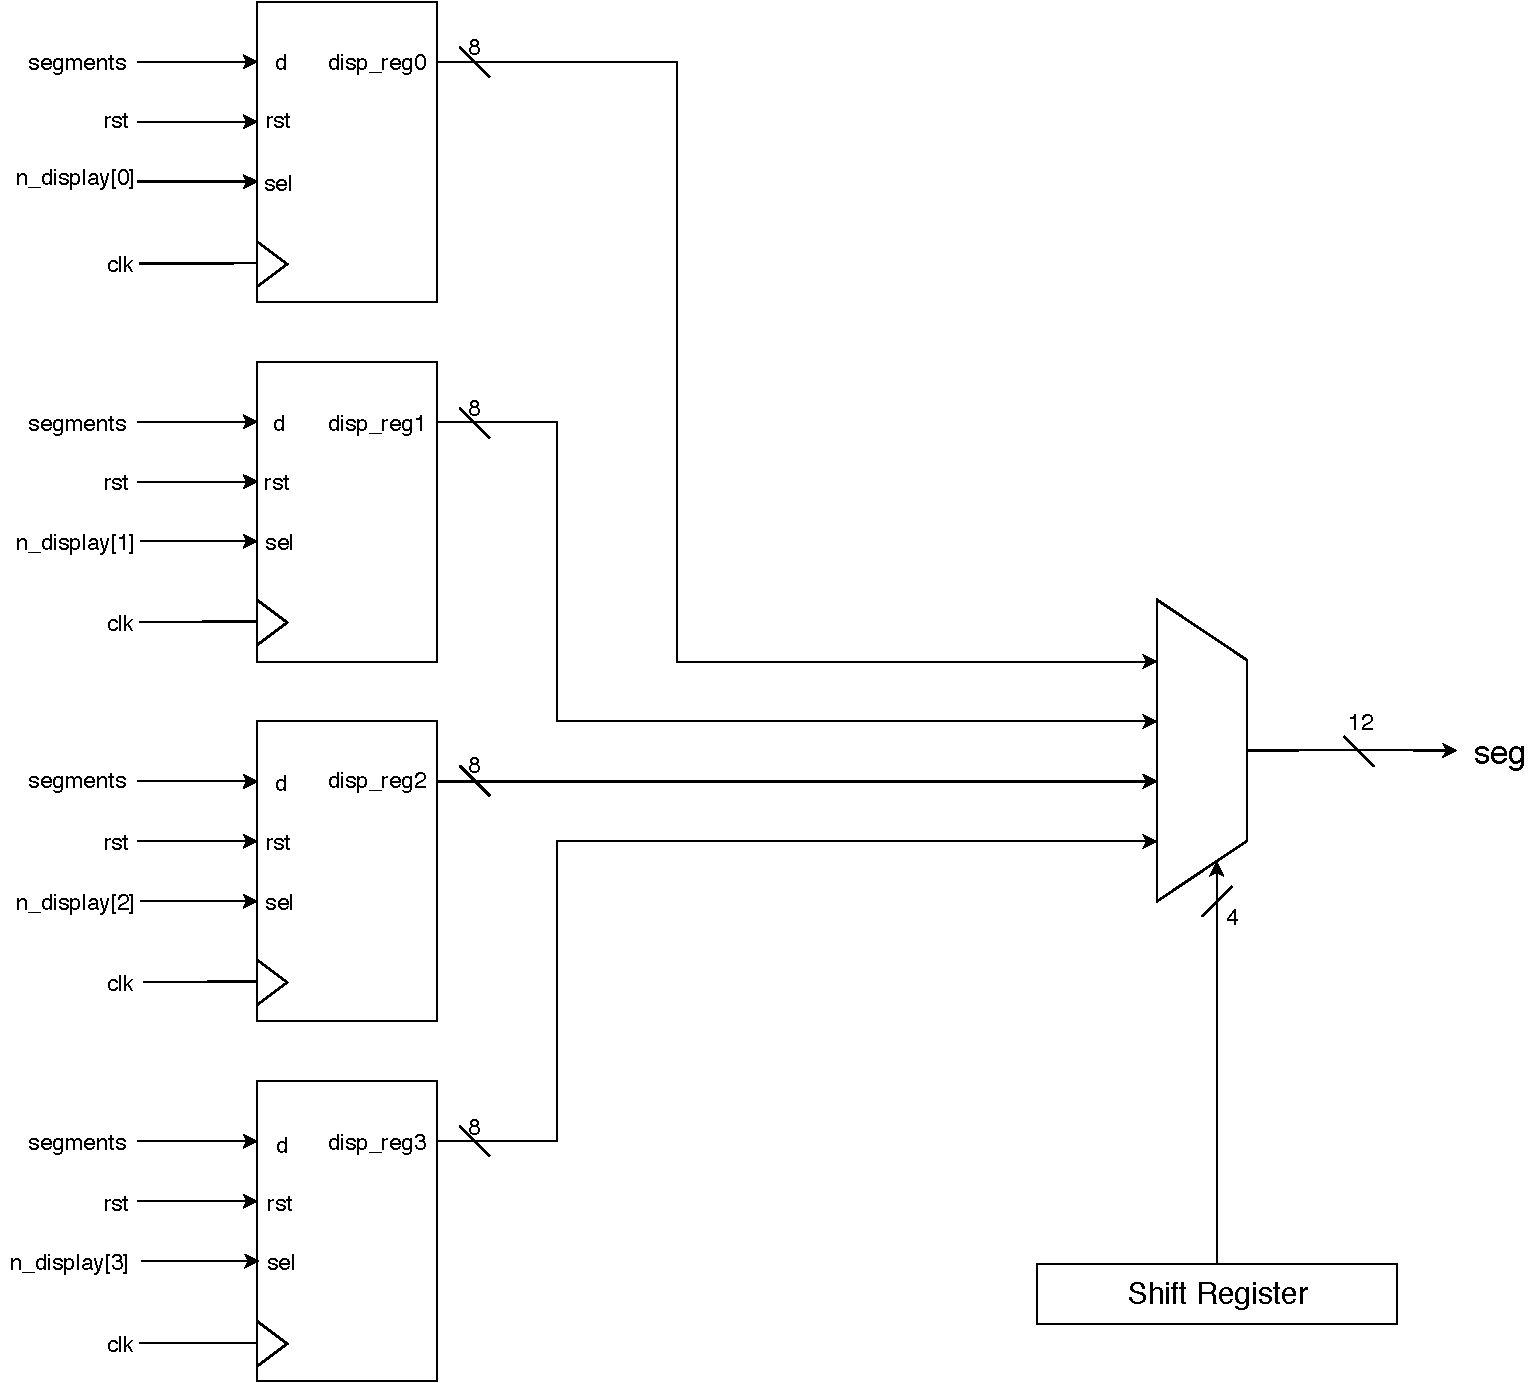
\includegraphics[scale=0.45]{display_interface}}
    \vspace{0cm}\caption{Block diagram of the display implementation.}
    \label{fig:display_interface}
\end{figure}

\clearpage
\subsection{Description of the buttons and switches peripheral}
\begin{figure}[!htbp]
    \centerline{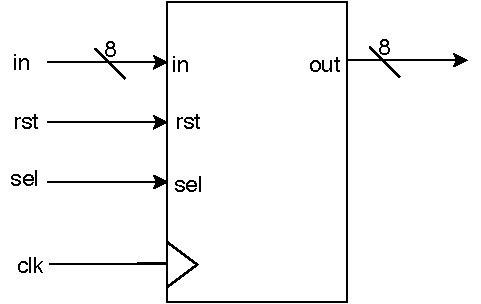
\includegraphics[scale=0.8]{switch_interface}}
    \vspace{0cm}\caption{Buttons and switches interface.}
    \label{fig:switch_interface}
\end{figure}

\subsection{Description of the LFSR peripheral}
Linear Feedback Shift Register (LFSR) shown in Figure~\ref{fig:LFSR}, it is a shift register 
whose input bit is a linear function of its previous state. The output from a standard shift register is fed back into its input in such a 
way as to cause the function to endlessly cycle through a sequence of patterns. Due the fact these circuit is simple to construct
and are useful on our application, it is used to generate the random sequences to the memory game.

\vspace{10pt}
\begin{figure}[!htbp]
    \centerline{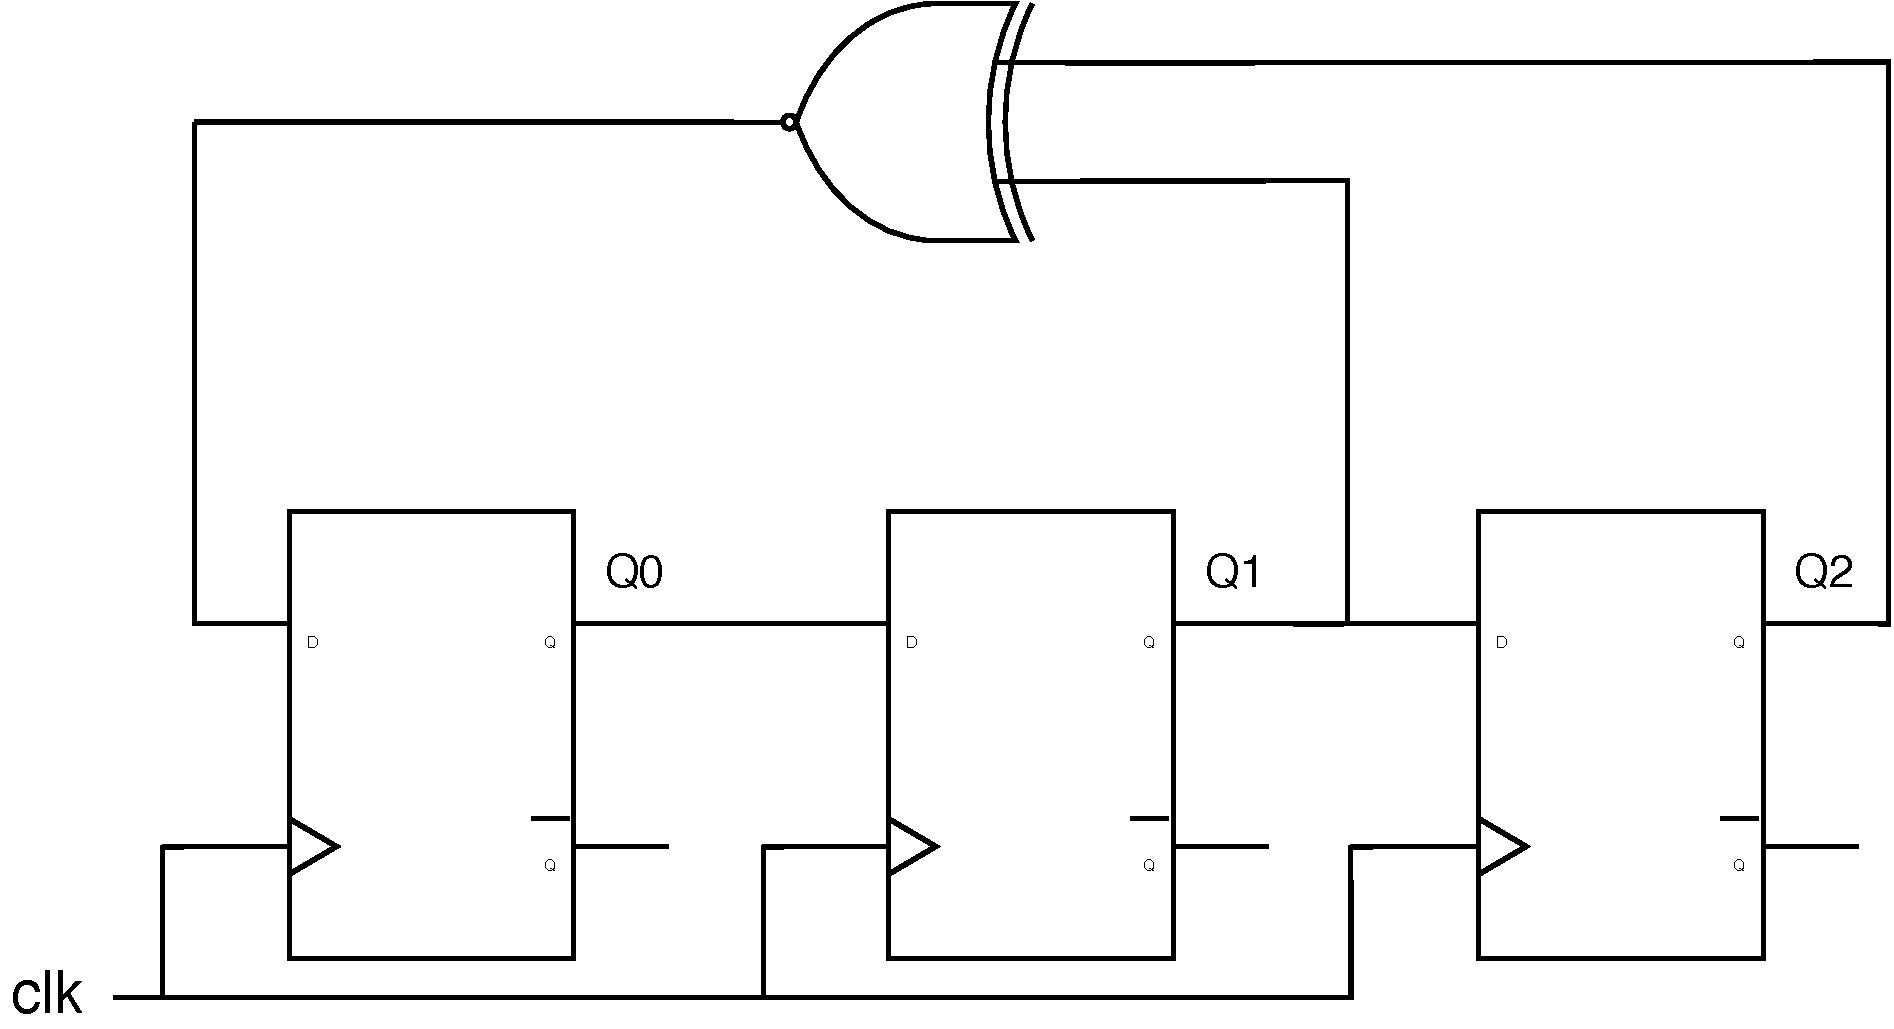
\includegraphics[scale=0.45]{LFSR}}
    \vspace{0cm}\caption{LFSR peripheral.}
    \label{fig:LFSR}
\end{figure}

\clearpage
\noindent The LFSR have 3 bits and the Table~\ref{tab:LFSR} shows the generation of multiple sequences contained in 
a range from [0:7]. During the development of this project we find some issues in the generation key of the game.
To resolve this problem we create a LUT with a size of 8 containing shuffled values (1,2,4,8) of the game LEDS,
finally we use the values produce by the LFSR to index this LUT to generate different sequences for the game.

\begin{table}[!htbp]
\centering
    \begin{tabular}{c|ccc}
        clk & $Q_0$ & $Q_1$ & $Q_2$ \\
        \hline
        - & 0 & 0 & 1 \\
        1 & 1 & 0 & 0 \\
        2 & 0 & 1 & 0 \\
        3 & 1 & 0 & 1 \\
        4 & 1 & 1 & 0 \\
        5 & 1 & 1 & 1 \\
        6 & 0 & 1 & 1 \\
        7 & 0 & 0 & 1 \\   
    \end{tabular}
    \caption{Truth table of the circuit LFSR.}
    \label{tab:LFSR}
\end{table} 

\section{Results}
\label{sec:results}

